\section{Discussion}
\label{sec:disc}

Having shown that regularization can improve the {\bf anchor} topic
modeling algorithm, in this section we discuss \emph{why} these regularizations can
improve the model and the implications for practitioners.

\paragraph{Efficiency}

Efficiency is a function of the number of iterations and the cost of
each iteration.  Both {\bf anchor} and {\bf anchor-$L_2$} require a
single iteration, although the latter's iteration is slightly more
expensive.  For {\bf beta}, as described in Section~\ref{sec:beta}, we
update anchor coefficients $C$ row by row, and then repeat the process
over several iterations until it converges.  However, it often
converges within ten iterations (Figure~\ref{fig:convergence}) on all
three datasets: this requires much fewer iterations than \abr{mcmc} or variational
inference, and the iterations are less expensive.  In addition, since
we optimize each row $C_{i,\cdot}$ independently, the algorithm can be
easily parallelized.

\begin{figure}[t!]
\centering
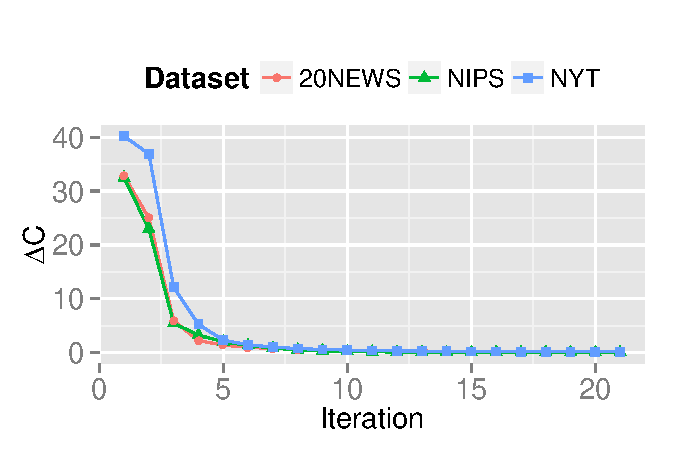
\includegraphics[width=\linewidth]{2014_acl_reganchor/figures/Convergence_C.pdf}
\caption{Convergence of anchor coefficient $C$ for {\bf anchor-beta}.
$\Delta C$ is the difference of current $C$ from the $C$ at the previous iteration.
$C$ is converged within ten iterations for all three datasets.}
\label{fig:convergence}
\end{figure}

\paragraph{Sensitivity to Document Frequency}

While the original {\bf anchor} is sensitive to the document frequency $M$
(Figure~\ref{fig:anchor-select}), adding regularization makes this less
critical.  Both {\bf anchor-$L_2$} and {\bf anchor-beta} are less sensitive to
$M$ than {\bf anchor}.

To highlight this, we compare the topics of {\bf anchor} and {\bf anchor-beta}
when $M=100$.  As Table~\ref{tab:sensitive-m} shows, the words
``article'', ``write'', ``don'' and ``doe'' appear in most of {\bf
  anchor}'s topics. While {\bf anchor-$L_2$} also has some bad
topics, it still can find reasonable topics, demonstrating {\bf
  anchor-beta}'s greater robustness to suboptimal $M$.



\begin{table*}[t!]
\begin{small}
   \begin{center}
\begin{tabular}{|c|p{6cm}|p{6cm}|} \hline
{\bf Topic} & {\bf anchor} & {\bf anchor-beta} \\ \hline
frequently & \green{article} \red{write} \blue{don} \purple{doe} make time people good file question & \green{article} \red{write} \blue{don} \purple{doe} make people time good email file \\ \hline
debate & \red{write} \green{article} people make \blue{don} \purple{doe} god key government time & people make god \green{article} \red{write} \blue{don} \purple{doe} key point government \\ \hline
wings & game team \red{write} wings \green{article} win red play hockey year & game team wings win red hockey play season player fan \\ \hline
stats & player team \red{write} game \green{article} stats year good play \purple{doe} & stats player season league baseball fan team individual playoff nhl \\ \hline
compile & program file \red{write} email \purple{doe} windows call problem run \blue{don} & compile program code file ftp advance package error windows sun \\ \hline
\end{tabular}

   \end{center}
\end{small}
\caption{Topics from {\bf anchor} and {\bf anchor-beta} with $M=100$ on \abr{20news} with 20 topics.
  Each topic is identified with its associated anchor word.
  When $M=100$, the topics of {\bf anchor} suffer: the four colored words appear in almost every topic.
  {\bf anchor-beta}, in contrast, is less sensitive to suboptimal $M$. }
\label{tab:sensitive-m}
\end{table*}


\paragraph{$L_2$ (Sometimes) Improves Generalization}

As Figure~\ref{fig:select-lambda} shows, {\bf anchor-$L_2$} sometimes
improves held-out development likelihood for the smaller
\abr{20news} corpus.  However, the $\lambda$ selected on development data does
not always improve test set performance.  This, in Figure~\ref{fig:results},
{\bf anchor-beta} closely tracks {\bf anchor}.  Thus, $L_2$ regularization does
not hurt generalization while imparting expressiveness and
robustness to parameter settings.

\paragraph{Beta Improves Interpretability}

Figure~\ref{fig:results} shows that {\bf anchor-beta} improves topic
interpretability (\abr{ti}) compared to unregularized anchor methods.
In this section, we try to understand why.

We first compare the topics from the original {\bf anchor} against {\bf
  anchor-beta} to analyze the topics qualitatively.
Table~\ref{tab:compare-beta} shows that {\bf beta} regularization promotes rarer
words within a topic and demotes common words.  For example, in the topic about
hockey with the anchor word \underline{game}, ``run'' and ``good''---ambiguous,
polysemous words---in the unregularized topic are replaced by ``playoff'' and
``trade'' in the regularized topic.  These words are less ambiguous and more
likely to make sense to a consumer of topic models.

Figure~\ref{fig:density-plot} shows why this happens.  Compared to the
unregularized topics from {\bf anchor}, the beta regularized topic steals from the rich and
creates a more uniform distribution.  Thus, highly frequent words do not as
easily climb to the top of the distribution, and the topics reflect topical,
relevant words rather than globally frequent terms.

\begin{figure*}[t!]
\centering
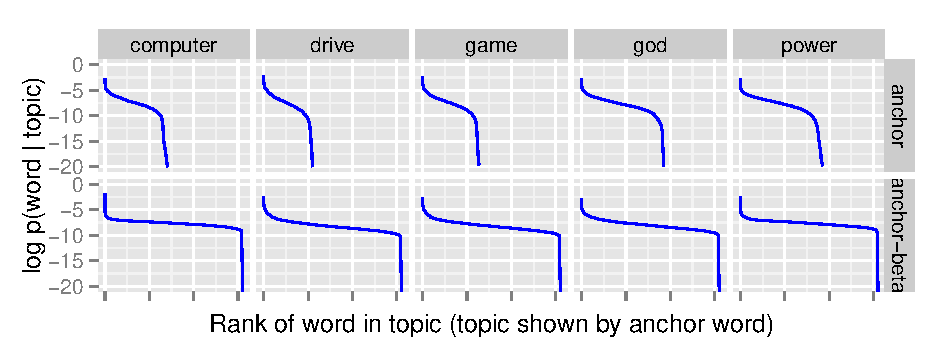
\includegraphics[width=0.9\linewidth]{2014_acl_reganchor/figures/density}
\caption{How beta regularization influences the topic distribution.  Each topic
  is identified with its associated anchor word.  Compared to the unregularized
  {\bf anchor} method, {\bf anchor-beta} steals
  probability mass from the ``rich'' and prefers a smoother distribution of
  probability mass.  These words often tend to be unimportant, polysemous words
  common across topics.
}
\label{fig:density-plot}
\end{figure*}

\begin{table*}[t!]
\begin{small}
   \begin{center}
       \begin{tabular}{|p{1.2cm}|c|p{8cm}|} \hline
           Topic & Shared Words & {\bf anchor} (Top, green) vs. {\bf anchor-beta} (Bottom, orange) \\ \hline
\multirow{2}{*}{computer}	&	\multirow{2}{4cm}{computer means science screen}	&	\cellcolor{green!30}system phone university problem doe work windows internet software chip mac set fax technology information data\\
&	&	\cellcolor{orange!30}quote mhz pro processor ship remote print devices complex cpu electrical transfer ray engineering serial reduce\\ \hline

\multirow{2}{*}{power}	&	\multirow{2}{4cm}{power play period supply ground light battery engine}	&	\cellcolor{green!30}car good make high problem work back turn control current small time\\
&	&	\cellcolor{orange!30}circuit oil wire unit water heat hot ranger input total joe plug\\ \hline
\end{tabular}

\begin{tabular}{|p{1.2cm}|c|p{5cm}|} \hline
\multirow{2}{*}{god}	&	\multirow{2}{7cm}{god jesus christian bible faith church life christ belief religion hell word lord truth love}	&	\cellcolor{green!30}people make things true doe\\
&	&	\cellcolor{orange!30}sin christianity atheist peace heaven\\ \hline

\multirow{2}{*}{game}	&	\multirow{2}{7cm}{game team player play win fan hockey season baseball red wings score division league goal leaf cup toronto}	&	\cellcolor{green!30}run good\\
&	&	\cellcolor{orange!30}playoff trade\\ \hline

\multirow{2}{*}{drive}	&	\multirow{2}{7cm}{drive disk hard scsi controller card floppy ide mac bus speed monitor switch apple cable internal port meg}	&	\cellcolor{green!30}problem work\\
&	&	\cellcolor{orange!30}ram pin\\ \hline
\end{tabular}

  \end{center}
\end{small}
\caption{Comparing topics---labeled by their anchor word---from {\bf
    anchor} and {\bf anchor-beta}. With beta regularization, relevant
  words are promoted, while more general words are suppressed,
  improving topic coherence.}
\label{tab:compare-beta}
\end{table*}